\documentclass[11pt,a4paper]{article}

% Packages
\usepackage[utf8]{inputenc}
\usepackage[spanish, es-tabla]{babel}
\usepackage{caption}
\usepackage{listings}
\usepackage{minted}
\usepackage{adjustbox}
\usepackage[colorlinks=true]{hyperref}
\usepackage[shortlabels]{enumitem}
\usepackage{boldline}
\usepackage{amssymb, amsmath}
\usepackage{amsthm}
\usepackage{subcaption}
\usepackage[noend]{algpseudocode}
\usepackage[margin=1in]{geometry}
\usepackage{xcolor}
\usepackage{soul}
\usepackage{upgreek}

%\usemintedstyle{bw}

\decimalpoint

\hypersetup{
  colorlinks=magenta
}

% Meta
\title{Procesos Estocásticos\\ \Large{Ejercicios 3} }
\author{Antonio Coín Castro}
\date{\today}

% Custom
\providecommand{\abs}[1]{\lvert#1\rvert}
\setlength\parindent{0pt}
% Redefinir letra griega épsilon.
\let\epsilon\upvarepsilon
% Fracciones grandes
\newcommand\ddfrac[2]{\frac{\displaystyle #1}{\displaystyle #2}}
% Primera derivada parcial: \pder[f]{x}
\newcommand{\pder}[2][]{\frac{\partial#1}{\partial#2}}

\newcommand{\fx}{\frac{1}{\sqrt{2\pi}\sigma} e^{\frac{-(x-\mu)^2}{2\sigma^2}}}
\newcommand{\R}{\mathbb{R}}

\begin{document}
\maketitle

\textbf{Ejercicio 1.} \textit{Considera el ejemplo de \textit{gambler's ruin} como cadena de Markov, donde en cada jugada se apuesta 1 euro, la banca tiene capital infinito, y el jugador tiene una probabilidad de $1/2$ de ganar en cada jugada.}
\textit{
\begin{itemize}
  \item[(i)] Hacer una gráfica del número medio de jugadas que el jugador puede hacer antes de arruinarse, en función del dinero inicial.
  \item[(ii)] Estimar media y varianza con 20 ejecuciones considerando un dinero inicial de $1,2,\dots, 50$ euros. ¿Cómo varían la media y la varianza cuando aumenta el dinero inicial?
\end{itemize}
}

\textit{Solución}. La cadena de Markov con infinitos estados que representa este juego es la siguiente:

\begin{figure}[h!]
  \centering
  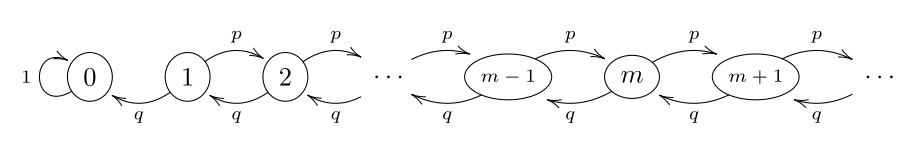
\includegraphics[width=.8\textwidth]{img/gambler.jpg}
\end{figure}

Las cantidades que queremos estimar son $k_m := \mathbb E_m[t \text{ to } 0]$, $m\ge 0$. Sabemos que estos valores pueden calcularse teóricamente como las soluciones minimales no negativas del sistema:
\[
\begin{cases}
  k_0 = 0\\
  k_m = 1 + \frac{1}{2}k_{m-1} + \frac{1}{2}k_{m+1}, & m\ge 1.
\end{cases}
\]

Si resolvemos esta ecuación en recurrencia (teniendo en cuenta la condición inicial), obtenemos que la solución general es de la forma
\[
k_m = mA - m^2 + m, \quad m \ge 0.
\]

Ahora, como debe ser $k_m\ge 0$ para todo $m$, necesariamente debe ser $A=\infty$, por lo que concluimos que $k_m=\infty$ para todo $m\ge 1$. Es decir, aunque sabemos que nos arruinaremos con probabilidad $1$, el número de jugadas esperadas para que esto ocurra es $\infty$, independientemente de nuestro dinero inicial (salvo que empecemos sin dinero).\\

A la hora de hacer una simulación para estimar las $k_m$ debemos tener cuidado, pues como hemos visto teóricamente, no convergerán a ningún valor por mucho que repitamos el experimento. Tenemos en primer lugar una clase que representa la cadena de Markov asociada al juego:

\begin{minted}{python}
import numpy as np
from scipy.stats import uniform
import matplotlib.pyplot as plt

class GamblersRuin:
    def __init__(self, p, m_ini):
        """ The infinite chain is represented by the probability of winning
            a round ('p') and the initial money ('m_ini'). """

        self.p = p
        self.m_ini = m_ini
        self.m = m_ini

    def step(self):
        """ Simulate a single step in the chain and return the new state. """
        if self.m == 0:
            return 0
        u = uniform.rvs()
        self.m = self.m + 1 if u <= self.p else self.m - 1
        return self.m
\end{minted}

Escribimos ahora una función que simule una cadena desde un estado inicial dado, y cuente los pasos necesarios para arruinarse. En caso de alcanzar el límite de iteraciones y no haberse arruinado ($10^5$ pasos), devolvemos justamente este límite de iteraciones, pues consideramos que es un número suficientemente grande como para simbolizar lo que queremos (es decir, que $k_m=\infty$). Debemos fijar un límite porque de otro modo cabría la posibilidad de que la simulación nunca acabase.

\begin{minted}{python}
def steps_to_ruin(m_ini, t):
    """ Compute the steps performed until going bankrupt, with up to t iterations
        of the chain starting at m_ini. If the bankrupt state fails to be reached,
        the total number of iterations of the chain is returned. """

    if m_ini == 0:
        return 0.0
    MC = GamblersRuin(0.5, m_ini)
    for tt in range(1, t + 1):
        if MC.step() == 0:
            return tt
    return t
\end{minted}

Ejecutamos ahora esta función con 20 cadenas, para cada estado inicial $1,2,\dots, 50$. En cada estado calculamos la media y la varianza muestral de las 20 cadenas, estimando efectivamente los valores de $k_m$ y su varianza.


\begin{minted}{python}
np.random.seed(1)
N = 20
M = 50
ms = np.arange(1, M + 1)
T = int(1e5)
ruin_time = np.zeros((M, N))
for m in ms:
    ruin_time[m - 1] = [steps_to_ruin(m, T) for _ in range(N)]
mean_rt = np.mean(ruin_time, axis = 1)
var_rt = np.var(ruin_time, axis = 1)
\end{minted}

Obtenemos unas gráficas como las siguientes:
\newpage

\begin{figure}[h!]
  \centering
  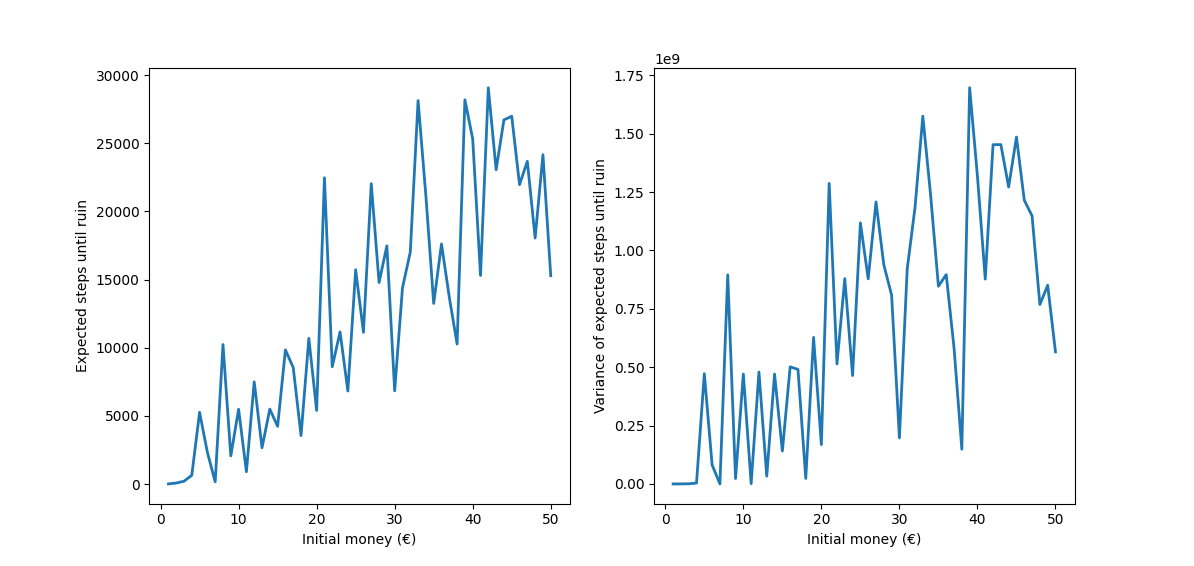
\includegraphics[width=.95\textwidth]{img/gambler_mean_var}
  \caption{Estimación de la media y varianza del número de jugadas hasta arruinarse, en función del dinero inicial.}
\end{figure}

\begin{figure}[h!]
  \centering
  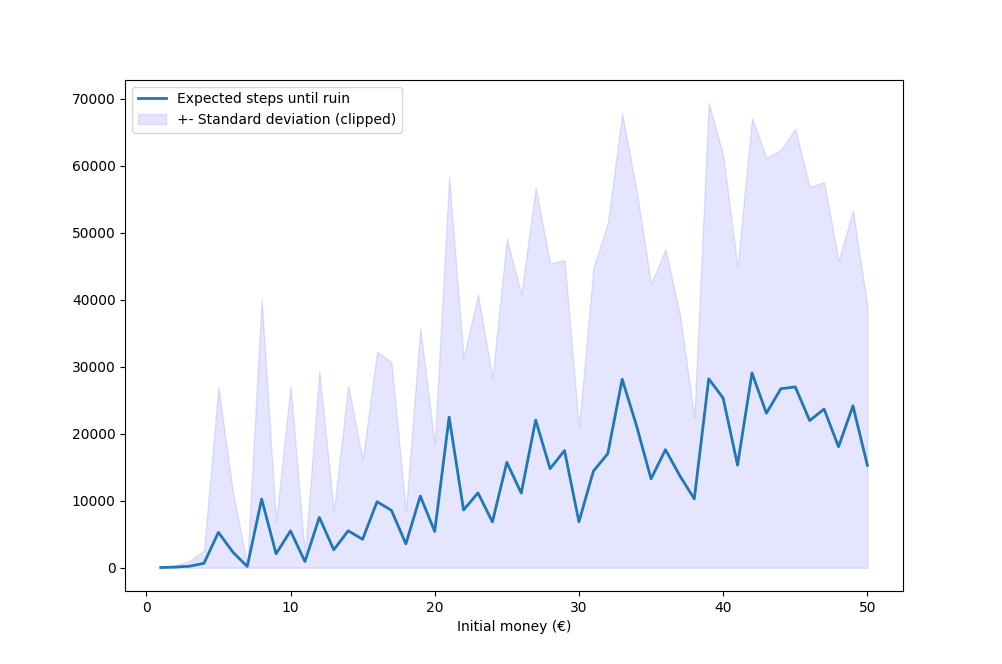
\includegraphics[width=.7\textwidth]{img/gambler_ci}
  \caption{Representación de $\hat k_m \pm \sigma_m$, donde $\sigma_m$ es la desviación típica muestral de 20 ejecuciones, truncada inferiormente en $0$.}
  \label{fig:std}
\end{figure}

Podemos observar que, como adelantábamos, el hecho de que teóricamente $k_m$ sea infinito introduce mucha variabilidad en las simulaciones. En particular, la media parece seguir una tendencia creciente en función del dinero inicial, llegando a tomar valores de hasta casi 30000 jugadas, pero presenta muchos picos que hacen que la transición de una cantidad inicial a otra no sea suave. La varianza es muy grande en todos los casos (la escala de la gráfica es $10^9$), y observamos también que parece aumentar con el dinero inicial. Esto tiene sentido, ya que aunque $k_m=\infty$ para todo $m\ge 1$, será más difícil llegar al estado $0$ conforme más lejos de él empecemos, pero si en alguna de las simulaciones o bien se consigue en pocos pasos o bien no se llega a conseguir, la varianza crecerá considerablemente.\\

El comportamiento de la media y la varianza (o desviación típica) se observa bastante bien en la Figura \ref{fig:std}, donde se ve claramente la tendencia creciente de ambos estimadores frente al dinero inicial.

\textbf{Ejercicio 2.} \textit{Indicar cuáles de las siguientes matrices, si son usadas como matrices de un sistema dinámico a tiempo discreto, son}
\textit{
\begin{enumerate}[a)]
  \item estables (todos los autovalores tienen $|\lambda|<1$),
  \item inestables (hay al menos un autovalor con $|\lambda| >1$),
  \item marginales (hay al menos un autovalor con $|\lambda|=1$ y los demás tienen $|\lambda|<1$),
  \item oscilantes (hay al menos un autovalor con $\lambda=-1$ y los demás tienen $|\lambda|<1$).
\end{enumerate}
}
\textit{Indicar los autovalores y los autovectores correspondientes a las componentes estables, inestables, marginales y oscilantes.}

\[
  A =
  \begin{pmatrix}
    0.175  & 0.125  & 0.725  & -0.225 \\
    0.125  & 0.175  & -0.225 &  0.725 \\
    0.725  & -0.225 & 0.175  &  0.125 \\
    -0.225 & 0.725  & 0.125  & -0.175 \\
  \end{pmatrix}
  \quad
  B =
  \begin{pmatrix}
     0.30 & -0.30 &  0.95 & -0.45 \\
    -0.30 &  0.30 & -0.45 &  0.95 \\
     0.95 & -0.45 &  0.30 & -0.30 \\
    -0.45 &  0.95 & -0.30 &  0.30 \\
  \end{pmatrix}
\]
\[
  C =
  \begin{pmatrix}
     0.05 & -0.05 &  0.70 & -0.20 \\
    -0.05 &  0.05 & -0.20 &  0.70 \\
     0.70 & -0.20 &  0.05 & -0.05 \\
    -0.20 &  0.70 & -0.05 &  0.05 \\
  \end{pmatrix}
  \quad
  D =
  \begin{pmatrix}
    -0.125 & -0.125 &  0.775 & -0.025 \\
    -0.125 & -0.125 & -0.025 &  0.775 \\
     0.775 & -0.025 & -0.125 & -0.125 \\
    -0.025 &  0.775 & -0.125 & -0.125 \\
  \end{pmatrix}
\]
\vspace{.5em}

\textit{Solución}. Escribimos una función que decida el tipo de estabilidad de cada matriz, ayudándonos de \verb|numpy|:

\begin{minted}{python}
import numpy as np
def compute_stability(M):
    """ Decides on the stabilty of the dicrete time linear dynamical
        system based on the matrix 'M'. """

    ls, vs = np.linalg.eig(M)
    ls = np.round(ls, decimals = 5)
    ls_abs = np.abs(ls)
    if (ls_abs < 1).all():
        return "stable", ls, vs
    if (ls_abs > 1).any():
        return "unstable", ls[ls_abs > 1], vs[:, ls_abs > 1]
    if (ls == -1).any() and (ls_abs[ls != -1] < 1).all():
        return "oscillatory stable", ls[ls == -1], vs[:, ls == -1]
    if (ls_abs == 1).any() and (ls_abs[ls_abs != 1] < 1).all():
        return "marginally stable", ls[ls_abs == 1], vs[:, ls_abs == 1]
\end{minted}

Si escribimos nuestras matrices en el programa y las pasamos a la función, obtenemos directamente la respuesta al ejercicio:
\begin{verbatim}
The system associated with A is unstable
The unstable components are:
l1 = -1.00938
v1 = [-0.43012  0.5039   0.42418 -0.61738]
------
The system associated with B is unstable
The unstable components are:
l1 = 2.0
v1 = [ 0.5 -0.5  0.5 -0.5]
------
The system associated with C is marginally stable
The marginally stable components are:
l1 = 1.0
v1 = [ 0.5 -0.5  0.5 -0.5]
------
The system associated with D is oscillatory stable
The oscillatory stable components are:
l1 = -1.0
v1 = [-0.5 -0.5  0.5  0.5]
------
\end{verbatim}

\textit{Nota:} los autovectores están normalizados para que tengan módulo $1$. Además, con la definición que hemos dado, todo sistema oscilatorio es marginal (toda componente oscilatoria es marginal), por lo que el sistema $D$ también es marginal, con las mismas componentes marginales que oscilantes.\\

\textbf{Ejercicio 3}. \textit{Consideramos el sistema dinámico}
\begin{align*}
  x_{t+1}&=Ax_t + Bu_t + w_t,\\
  z_t &=Cx_t + v_t,
\end{align*}

\textit{donde}
\[
  A =
  \begin{pmatrix}
     0.15 &  0.15 &  0.70 & -0.20 \\
     0.15 &  0.15 & -0.20 &  0.70 \\
     0.70 & -0.20 &  0.15 &  0.15 \\
    -0.20 &  0.70 &  0.15 & -0.15 \\
  \end{pmatrix},
  \quad
  B =
  \begin{pmatrix}
    1.0 & 1.0 & 1.0 & 1.0
  \end{pmatrix}',
  \quad
  C =
  \begin{pmatrix}
    1.0 & 0.0 & 0.0 & 0.0 \\
    0.0 & 1.0 & 0.0 & 0.0
  \end{pmatrix}.
\]
\textit{Suponer que $w$ es un ruido Gaussiano con media $0$ y desviación típica igual a $\sigma_w=10$, y que $v$ es un ruido Gaussiano con media $0$ y desviación típica $\sigma_v$ (ambos con componentes independientes e idénticamente distribuidas). Crear un filtro de Kalman para estimar el estado de este sistema y hacer un gráfico del error
\[
e(t)=\sum_{k}(\hat x_{t,k} - x_{t,k})^2
\]
para $t=1,\dots,100$, en los dos casos en que $\sigma_v=1$ y $\sigma_v=10$.}\\

\textit{Solución}. Podemos dividir un paso del filtro de Kalman en dos etapas:\\

\textbf{Predict}
\begin{enumerate}
  \item[\textit{(i)}] \textit{Update prior for estimate: $\bar x_{t+1} = A\hat x_t + Bu_t$}
  \item[\textit{(ii)}] \textit{Update prior for covariance: $\bar P_{t+1}=AP_tA' + Q$}
\end{enumerate}

\textbf{Update}
\begin{enumerate}
  \item[\textit{(iii)}] \textit{Compute Kalman gain: $K_t = \bar P_t C'(C\bar P_tC' + R)^{-1}$}
  \item[\textit{(iv)}] \textit{Update estimate: $\hat x_{t} = \bar x_t + K_t(z_t - C\bar x_t)$}
  \item[\textit{(v)}] \textit{Update covariance: $P_t=(I -K_tC)\bar P_t$}
\end{enumerate}

Antes de mostrar el código implementado, hacemos una serie de consideraciones sobre el modelo:

\begin{enumerate}
  \item Para la primera iteración necesitamos los valores \textit{a priori} de $x_1$ y $P_1$. Como no tenemos ninguna información sobre el proceso, escogemos por ejemplo $\bar x_1=0$ y $\bar P_1=\sigma_w^2I$ (las varianzas de los errores iniciales son grandes, ya que no podemos evaluar cómo de buena es la aproximación $\bar x_1$). Esta elección inicial influye únicamente en la velocidad de convergencia y no en la bondad de las aproximaciones a largo plazo.
  \item En la expresión de $K_t$ interviene el cálculo de una inversa. Para aumentar la estabilidad podemos reescribir la ecuación como un sistema lineal $K_t(C\bar P_tC' + R)=\bar P_tC'$. Sin embargo, como la mayoría de \textit{solvers} numéricos resuelven sistemas de la forma $Ax=b$, calcularemos en su lugar la solución de $(C\bar P_tC' + R)'K_t' = C\bar P_t'$ y luego traspondremos el resultado. Sin embargo, como $\bar P_t$ y $R$ son simétricas (al ser matrices de covarianza), obtenemos que el sistema se simplifica como
  \[
  (C\bar P_tC' + R)K_t' = C\bar P_t.
  \]
  \item Como los ruidos Gaussianos $w$ y $v$ tienen componentes i.i.d, podemos suponer que siguen una normal multivariante de media $0$ y matrices de covarianza $10^2I$ y $\sigma_v^2I$, respectivamente. Para extraer valores de estas distribuciones usaremos la librería \verb|scipy.stats|.
  \item Para actualizar las estimaciones necesitamos conocer el valor de las variables observables $z_t$, que a su vez dependen del proceso oculto $x_t$. Es por esto que en el código debemos simular el proceso $x_t$ hasta el paso que nos interese, y utilizarlo en la fórmula de $z_t$ para simular las observaciones. Como valor inicial del proceso utilizaremos de nuevo el vector nulo.
  \item Tenemos libertad para elegir \textit{inputs} $u_t$ en cada instante de tiempo. Establecemos por ejemplo $u_t=1$ para todo $t$.
  \item Para disminuir la variabilidad de los cálculos aleatorios (debidos al ruido) realizamos varias iteraciones independientes del filtro, y calculamos la media de los errores obtenidos en cada una de ellas.
\end{enumerate}

Hechas estas consideraciones, implementamos el filtro de Kalman como un algoritmo iterativo, donde vamos realizando los pasos de predicción y actualización. El código desarrollado es el siguiente:

\begin{minted}{python}
import numpy as np
from scipy.linalg import solve
from scipy.stats import multivariate_normal
import matplotlib.pyplot as plt

np.random.seed(42)

def kf_predict_step(A, B, Q, u, xpred, P):
    """ Perform one step of the prediction phase. """

    xbar = A @ xpred + B @ u
    Pbar = A @ P @ A.T + Q
    return xbar, Pbar

def kf_update_step(C, Pbar, R, x, v, xbar):
    """ Perform one step of the update phase. """

    n = C.shape[1]
    K = solve(C @ Pbar @ C.T + R, C @ Pbar).T
    z = C @ x + v.rvs()
    xpred = xbar + K @ (z - C @ xbar)
    P = (np.diag(np.ones(n)) - K @ C) @ Pbar
    return K, xpred, P

def kf(A, B, C, Q, R, xs, us, xbar_0, Pbar_0, max_t):
    """ Perform 'max_t' iterations of the Kalman filter.
          - A, B: hidden process dynamics matrices.
          - C: observable process dynamics matrix.
          - xs: vector of actual hidden process values to simulate z_t.
          - us: vector of user-defined inputs.
          - xbar_0: prior of first value.
          - Pbar_0: prior of first covariance matrix.
          - Q: white noise covariance matrix for hidden process.
          - R: white noise covariance matrix for observable process. """

    n = A.shape[0]
    v = multivariate_normal(None, R, allow_singular = True)
    # A priori estimations
    Pbar = Pbar_0
    xbar = xbar_0
    # Array to store predictions
    xpreds = np.zeros((max_t, n))
    # Loop through iterations
    for t in range(max_t):
        K, xpred, P = kf_update_step(C, Pbar, R, xs[t], v, xbar)
        xbar, Pbar = kf_predict_step(A, B, Q, us[t], xpred, P)
        xpreds[t] = xpred
    return xpreds
\end{minted}

Para simular el proceso $x_t$ disponemos también de una función:

\begin{minted}{python}
def dynamical_system(A, B, us, Q, x0, max_t):
    """ Compute 'max_t' steps of the process defined by
            x_0 = x0,
            x_{t+1} = Ax_t + Bu_t + w_t,
        where w_t is a white Gaussian noise with covariance matrix Q. """

    n = A.shape[0]
    xs = np.full((max_t + 1, n), x0)
    w = multivariate_normal(None, Q, allow_singular = True)
    for t in range(1, max_t + 1):
        xs[t] = A @ xs[t - 1] + B @ us[t - 1] + w.rvs()
    return xs[1:]
\end{minted}

Ahora, establecemos los parámetros del sistema y realizamos varias ejecuciones independientes, midiendo en cada una el error en cada instante con respecto a los valores simulados de $x_t$. Lo hacemos para los distintos valores de $\sigma_v=1$ y $\sigma_v=10$.

\begin{minted}{python}
# Number of iterations
max_t = 100
ts = np.arange(max_t)
# Dynamics matrices
A = np.array([[0.15, 0.15, 0.70, -0.20],
             [0.15, 0.15, -0.20, 0.70],
             [0.70, -0.20, 0.15, 0.15],
             [-0.20, 0.70, 0.15, -0.15]])
B = np.array([1.0, 1.0, 1.0, 1.0]).reshape(-1, 1)
C = np.array([[1.0, 0.0, 0.0, 0.0],
             [0.0, 1.0, 0.0, 0.0]])
n = A.shape[0]
q = C.shape[0]
# Input signals are always 1 (irrelevant)
us = np.ones(max_t).reshape(-1, 1)
# White noise covariance matrices for hidden and observable states
sigma_w = 10.0
sigma_v = 1.0
Q = np.diag(np.full(n, sigma_w ** 2))
R = np.diag(np.full(q, sigma_v ** 2))
# Initial estimates
xbar_0 = np.zeros(n)
Pbar_0 = np.diag(np.full(n, sigma_w ** 2))
# Simulate system to get a sample
xs = dynamical_system(A, B, us, Q, xbar_0, max_t)
# Perform simulations of Kalman filters
runs = int(sigma_v * 10)
xpreds_runs = np.zeros((runs, max_t, n))
for i in range(runs):
    xpreds_runs[i] = kf(A, B, C, Q, R, xs, us, xbar_0, Pbar_0, max_t)
# Compute mean values
xpreds = np.mean(xpreds_runs, axis = 0)
errors = [np.linalg.norm(xs[t] - xpreds_runs[:, t], axis = 1) ** 2 for t in ts]
mean_error = np.mean(errors, axis = 1)
std_error = np.std(errors, axis = 1) / np.sqrt(runs)
\end{minted}


Hacemos una gráfica de las 4 componentes del sistema real y de las predicciones, para ver cómo de buena es la estimación (tomamos los valores medios de todas las ejecuciones del filtro). Los resultados se pueden observar en las Figuras \ref{fig:comp1} y \ref{fig:comp2}. Como vemos, para las dos primeras componentes las predicciones son bastante acertadas, mientras que las dos últimas tienen más error. Esto tiene sentido, ya que debido a la forma de la matriz $C$, en el proceso $z_t$ solo observamos las dos primeras componentes del sistema (perturbadas por el ruido). En el caso de $\sigma_v=10$ la discordancia es más grande, incluso en las dos primeras componentes, ya que el ruido es bastante mayor.\\

En cuanto al error cuadrático entre las predicciones y los valores reales (Figuras \ref{fig:error1} y \ref{fig:error2}), vemos como es mayor para el caso de $\sigma_v=10$, y que en ninguno de los casos llega a converger a $0$, sino que oscila bastante. Esto es debido al alto valor del ruido en el proceso oculto ($\sigma_w=10$), que distorsiona bastante las mediciones. Junto a los errores medios pintamos la desviación típica de la media (que sabemos que se puede estimar como $s/\sqrt{R}$, donde $R$ es el número de ejecuciones independientes y $s$ la desviación típica muestral insesgada). Vemos cómo con tan solo 10 ejecuciones esta desviación típica es apenas imperceptible cuando $\sigma_v=1$, y que con 100 ejecuciones aún se observa cierto error cuando $\sigma_v=10$.
\newpage

\begin{figure}[h!]
    \centering
    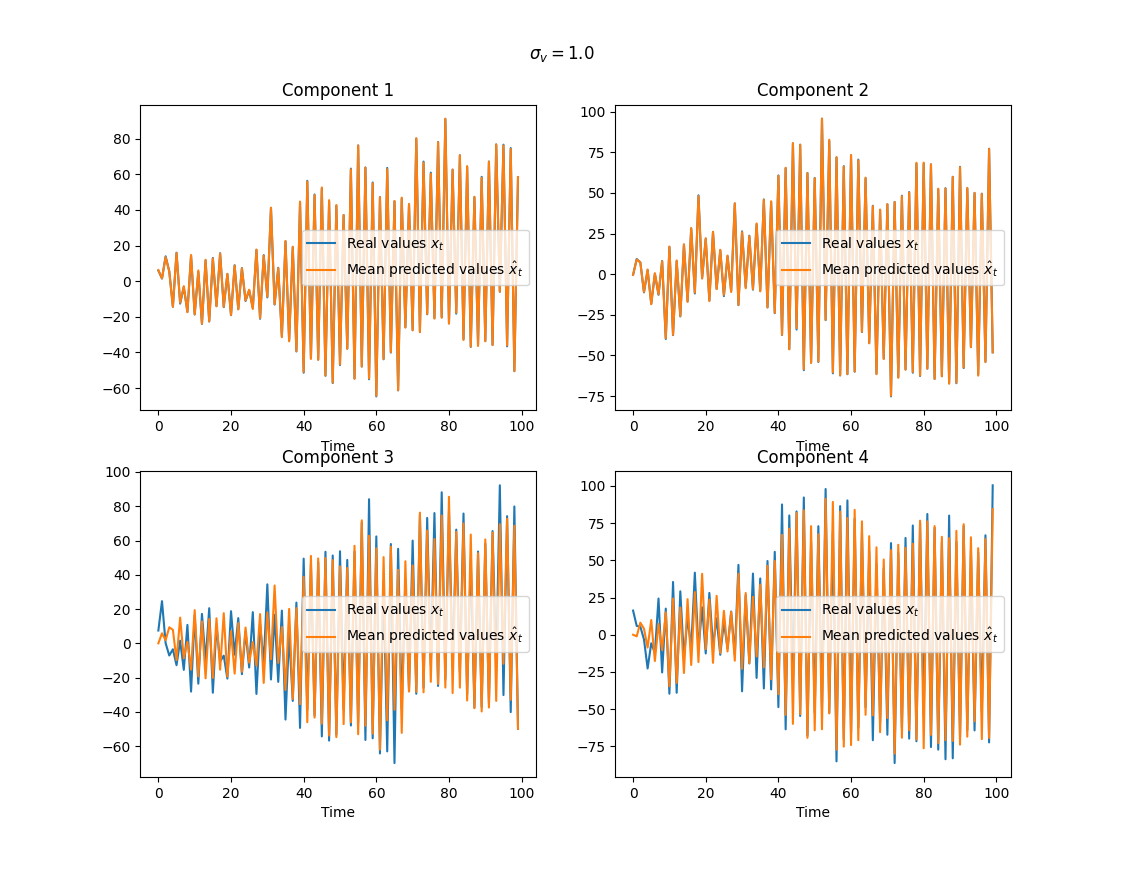
\includegraphics[width=.87\textwidth]{img/components_s1}
    \caption{Diferencia entre valores reales y predicciones medias para $\sigma_v=1$.}
    \label{fig:comp1}
\end{figure}

\begin{figure}[h!]
    \centering
    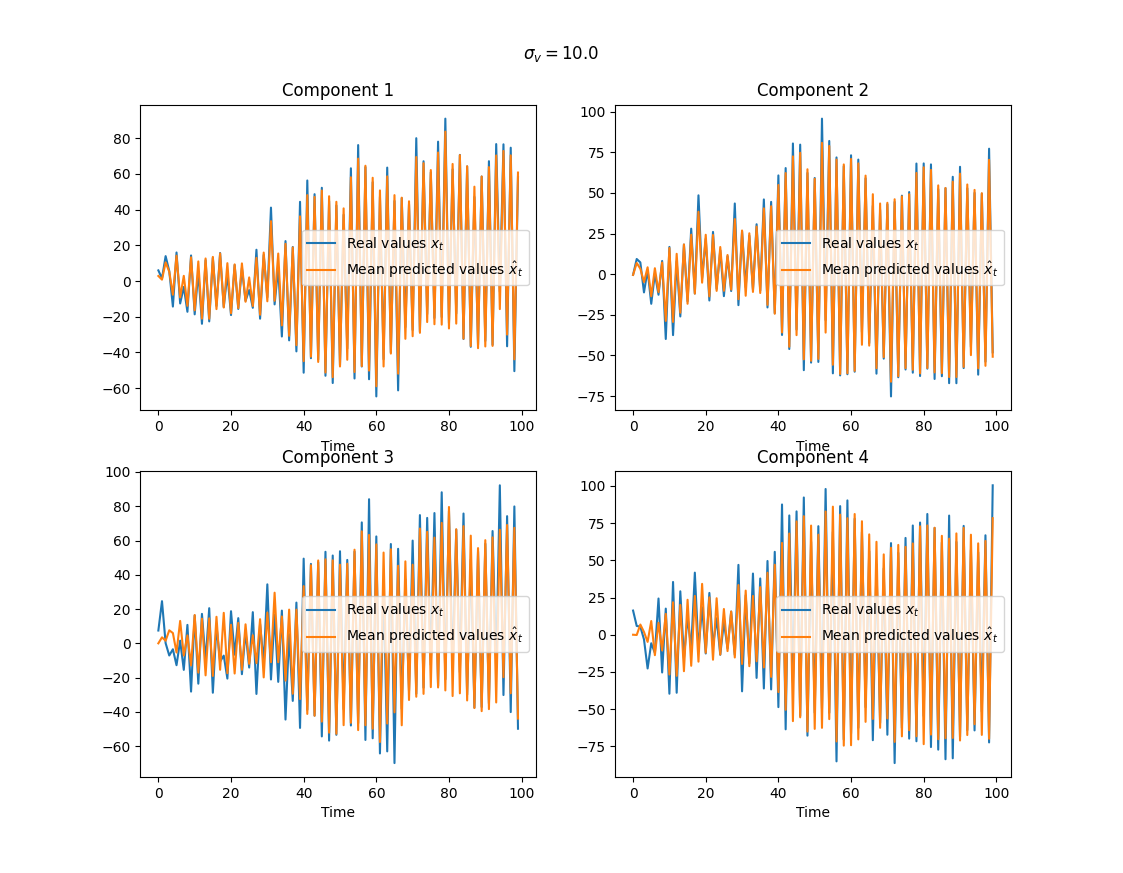
\includegraphics[width=.87\textwidth]{img/components_s10}
    \caption{Diferencia entre valores reales y predicciones medias para $\sigma_v=10$.}
    \label{fig:comp2}
\end{figure}

\newpage

\begin{figure}[h!]
    \centering
    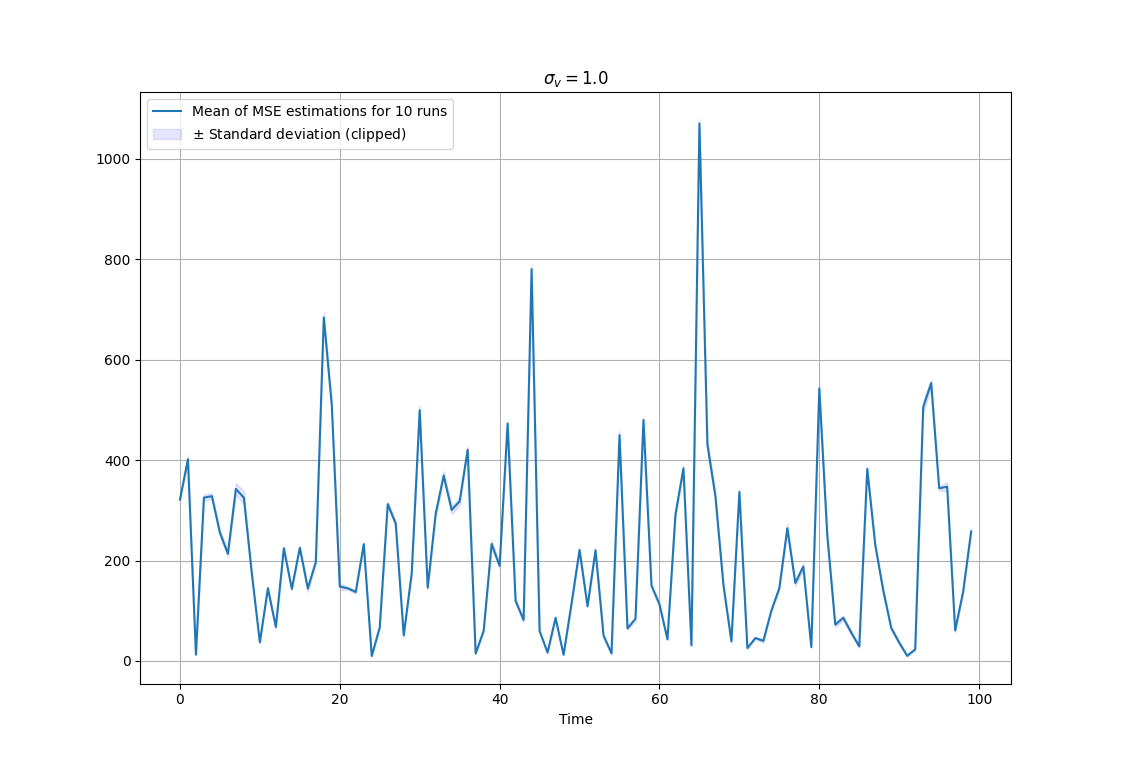
\includegraphics[width=.95\textwidth]{img/error_s1}
    \caption{Evolución del error cuadrático (promediado en todas las ejecuciones independientes) en función del tiempo, para $\sigma_v=1$.}
    \label{fig:error1}
\end{figure}

\begin{figure}[h!]
    \centering
    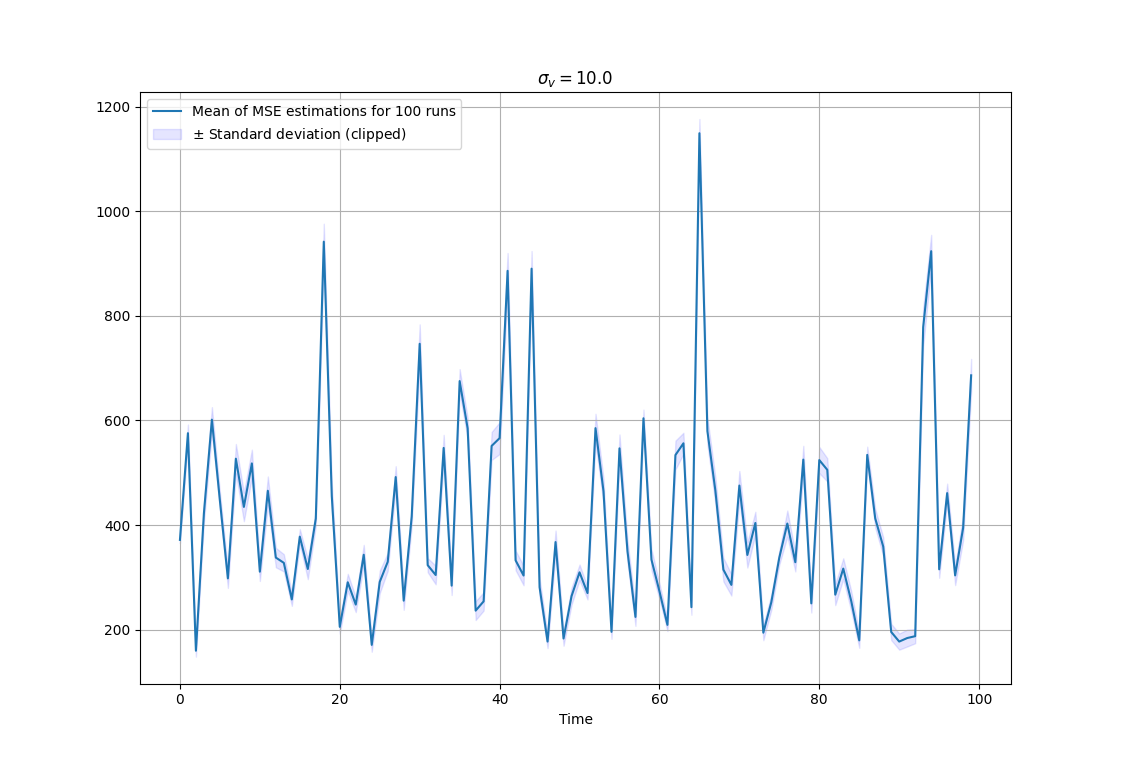
\includegraphics[width=.95\textwidth]{img/error_s10}
    \caption{Evolución del error cuadrático (promediado en todas las ejecuciones independientes) en función del tiempo, para $\sigma_v=10$.}
    \label{fig:error2}
\end{figure}

\newpage

Finalmente, hacemos una prueba para ver el error en la predicción si disminuimos el ruido de $w_t$. En particular, hacemos una gráfica del error en el caso extremo de $w_t \equiv 0$, es decir, sin ruido en el proceso oculto. Vemos como en este caso tras unas pocas iteraciones el error en la predicción del filtro converge a $0$, sin importar el valor de $\sigma_v$.

\begin{figure}[h!]
    \centering
    \begin{subfigure}{\textwidth}
        \centering
        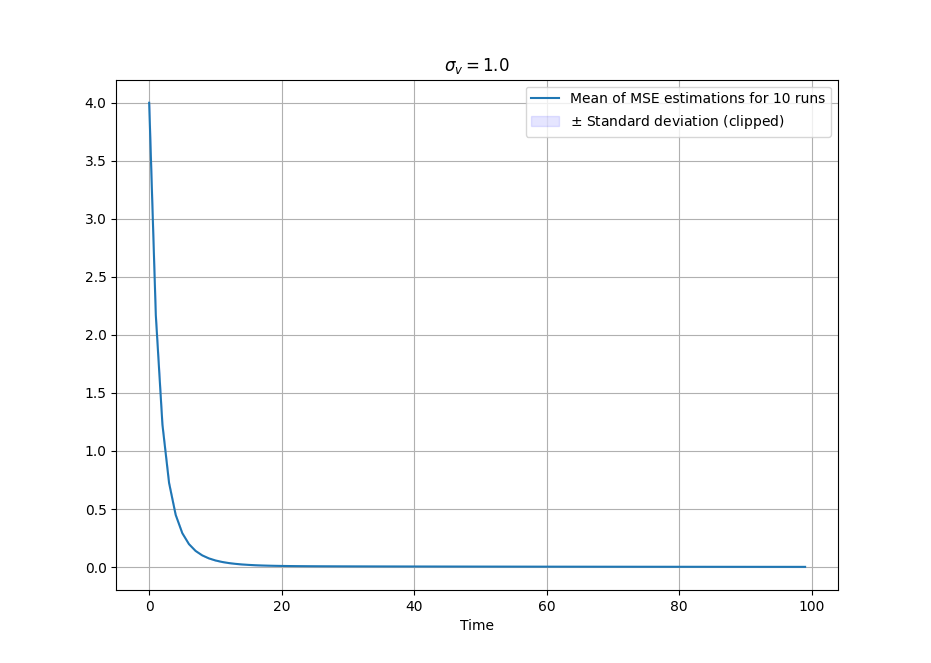
\includegraphics[width=.8\textwidth]{img/error_0noise}
    \end{subfigure}\\
    \begin{subfigure}{\textwidth}
        \centering
        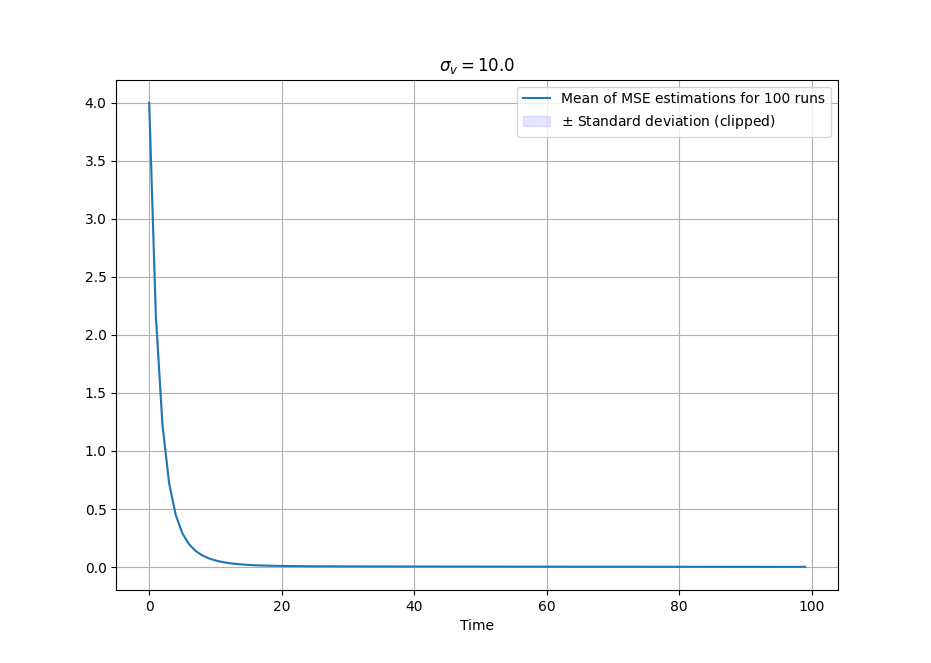
\includegraphics[width=.8\textwidth]{img/error_0noise_s10}
    \end{subfigure}
    \caption{Error medio para el caso sin ruido ($w_t\equiv 0$).}
    \label{fig:error0}
\end{figure}

\end{document}
